% Asset ID: AS1CoordinateGeometryCirclesTikZ-006
% Purpose: Two chord perpendicular bisectors meet at centre.
\documentclass[tikz,border=8pt]{standalone}
\usetikzlibrary{calc}
\begin{document}
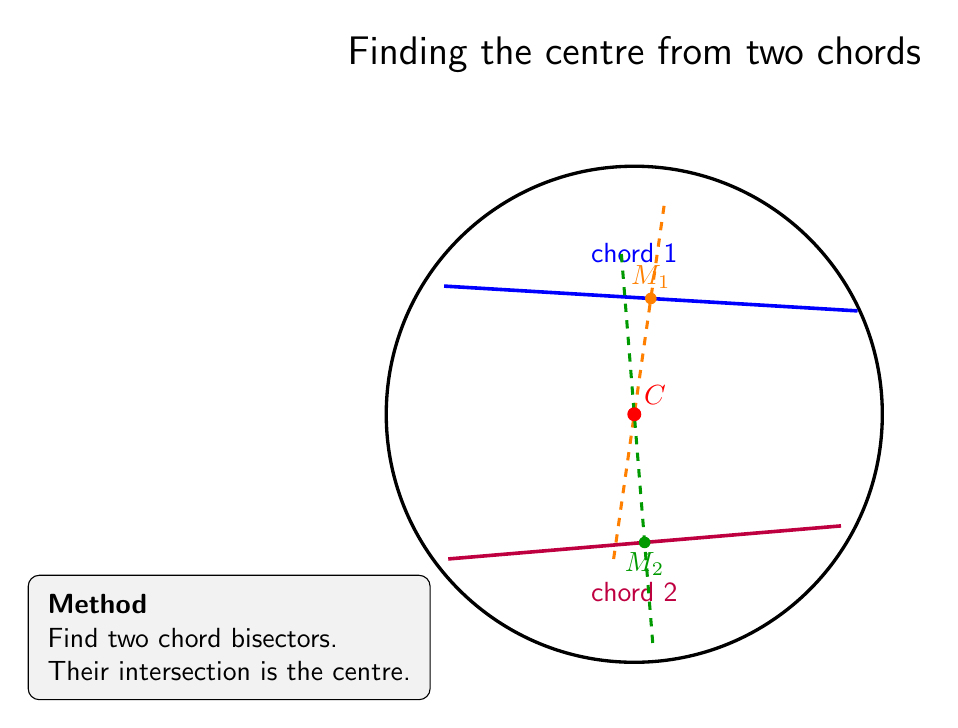
\begin{tikzpicture}[scale=1.05, font=\sffamily]
\node[align=center] at (0,4.35) {\Large Finding the centre from two chords};
\coordinate (O) at (0,0); \draw[line width=1.2pt] (O) circle (3);
\coordinate (A) at (-2.3,1.55); \coordinate (B) at (2.7,1.25); \draw[line width=1.3pt, blue] (A)--(B); \node[blue] at (0,1.95) {chord 1};
\coordinate (D) at (-2.25,-1.75); \coordinate (E) at (2.5,-1.35); \draw[line width=1.3pt, purple] (D)--(E); \node[purple] at (0,-2.15) {chord 2};
\coordinate (M1) at ($(A)!0.5!(B)$); \coordinate (M2) at ($(D)!0.5!(E)$); \fill[orange] (M1) circle (2pt) node[above] {$M_1$}; \fill[green!60!black] (M2) circle (2pt) node[below] {$M_2$};
\draw[line width=1.1pt, orange, dashed] ($(O)!-1.25!(M1)$)--($(O)!1.8!(M1)$); \draw[line width=1.1pt, green!60!black, dashed] ($(O)!-1.25!(M2)$)--($(O)!1.8!(M2)$);
\fill[red] (O) circle (2.4pt) node[above right] {$C$};
\node[align=left, draw, rounded corners, fill=gray!10, inner sep=7pt] at (-4.9,-2.7) {\textbf{Method}\\Find two chord bisectors.\\Their intersection is the centre.};
\end{tikzpicture}\end{document}
